\documentclass{common/sprawozdanie-agh}
\usepackage[utf8]{inputenc}
\usepackage[T1]{fontenc}
\usepackage{lmodern}
\usepackage{booktabs}
\usepackage{enumitem}
\usepackage{hyperref}
\usepackage{tabularx}
\usepackage{float}
\usepackage{amsmath}
\usepackage{graphicx}
\usepackage{tikz}
\usepackage{listings}
\usepackage{xcolor}
\usepackage{array}

\graphicspath{{common/}{figures/}}

\hypersetup{
    colorlinks=true,
    linkcolor=blue!60!black,
    urlcolor=blue!60!black,
    citecolor=blue!60!black
}

\usetikzlibrary{arrows.meta, positioning, shapes.geometric, calc}

% =====================================================================
% LISTING STYLES
% =====================================================================

% --- Common colors ---
\definecolor{codegreen}{rgb}{0,0.6,0}
\definecolor{codegray}{rgb}{0.5,0.5,0.5}
\definecolor{codepurple}{rgb}{0.58,0,0.82}
\definecolor{backcolour}{rgb}{0.95,0.95,0.92}
\definecolor{codeblue}{rgb}{0.13,0.29,0.53}
\definecolor{codeorange}{rgb}{0.8,0.4,0.0}

% --- Common literate for Polish characters ---
\newcommand{\polishliterate}{%
    literate=
    {ą}{{\k a}}1 {Ą}{{\k A}}1
    {ć}{{\'c}}1 {Ć}{{\'C}}1
    {ę}{{\k e}}1 {Ę}{{\k E}}1
    {ł}{{\l}}1 {Ł}{{\L}}1
    {ń}{{\'n}}1 {Ń}{{\'N}}1
    {ó}{{\'o}}1 {Ó}{{\'O}}1
    {ś}{{\'s}}1 {Ś}{{\'S}}1
    {ź}{{\'z}}1 {Ź}{{\'Z}}1
    {ż}{{\.z}}1 {Ż}{{\.Z}}1
}

% --- C style ---
\lstdefinestyle{cstyle}{
    language=C,
    backgroundcolor=\color{backcolour},
    commentstyle=\color{codegreen},
    keywordstyle=\color{codeblue}\bfseries,
    numberstyle=\tiny\color{codegray},
    stringstyle=\color{codepurple},
    directivestyle=\color{codeorange},
    basicstyle=\ttfamily\footnotesize,
    breakatwhitespace=false,
    breaklines=true,
    captionpos=b,
    keepspaces=true,
    numbers=left,
    numbersep=5pt,
    showspaces=false,
    showstringspaces=false,
    tabsize=4,
    morekeywords={uint32_t,uint64_t,int64_t,pcg32_random_t,
                  Individual,Gene,ProblemData,GAConfig,Event,
                  Room,Teacher,StudentGroup,Course,
                  MPI_Comm,MPI_Status,MPI_Datatype},
    \polishliterate
}

% --- Bash style ---
\lstdefinestyle{bashstyle}{
    language=bash,
    backgroundcolor=\color{backcolour},
    commentstyle=\color{codegreen},
    keywordstyle=\color{magenta},
    numberstyle=\tiny\color{codegray},
    stringstyle=\color{codepurple},
    basicstyle=\ttfamily\footnotesize,
    breakatwhitespace=false,
    breaklines=true,
    captionpos=b,
    keepspaces=true,
    numbers=none,
    showspaces=false,
    showstringspaces=false,
    tabsize=2,
    morekeywords={mpiexec,mpicc,make,gnuplot,source,export},
    \polishliterate
}

% --- Python style ---
\lstdefinestyle{pythonstyle}{
    language=Python,
    backgroundcolor=\color{backcolour},
    commentstyle=\color{codegreen},
    keywordstyle=\color{magenta},
    numberstyle=\tiny\color{codegray},
    stringstyle=\color{codepurple},
    basicstyle=\ttfamily\footnotesize,
    breakatwhitespace=false,
    breaklines=true,
    captionpos=b,
    keepspaces=true,
    numbers=left,
    numbersep=5pt,
    showspaces=false,
    showstringspaces=false,
    tabsize=4,
    \polishliterate
}

% --- Makefile style ---
\lstdefinestyle{makefilestyle}{
    language=make,
    backgroundcolor=\color{backcolour},
    commentstyle=\color{codegreen},
    keywordstyle=\color{codeblue}\bfseries,
    numberstyle=\tiny\color{codegray},
    stringstyle=\color{codepurple},
    basicstyle=\ttfamily\footnotesize,
    breakatwhitespace=false,
    breaklines=true,
    captionpos=b,
    keepspaces=true,
    numbers=none,
    showspaces=false,
    showstringspaces=false,
    tabsize=4,
    \polishliterate
}

% Default style
\lstset{style=cstyle}

% =====================================================================
% DOCUMENT
% =====================================================================
\begin{document}

\przedmiot{Systemy Równoległe i Rozproszone}
\tytul{Równoległy algorytm genetyczny}
\podtytul{do układania planu zajęć uniwersyteckich --- Projekt nr 26}
\kierunek{Informatyka Stosowana}
\wydzial{Fizyki i Informatyki Stosowanej}
\autor{Dawid Piotrowski, Jakub P.}
\data{Kraków, 2026}
\stronatytulowa{}
\tableofcontents
\newpage

% =====================================================================
% 1. WSTĘP
% =====================================================================
\section{Wstęp}

Problem układania planu zajęć uniwersyteckich (ang.~\textit{University Course Timetabling Problem}, UCTP) polega na przydzieleniu zdarzeń dydaktycznych do slotów czasowych i~sal, z~uwzględnieniem szeregu ograniczeń. Jest to problem NP-trudny --- przestrzeń rozwiązań rośnie wykładniczo z~liczbą zdarzeń, sal i~slotów czasowych~\cite{banczyk}.

Algorytmy genetyczne (AG) są skuteczną metaheurystyką do rozwiązywania UCTP, jednak czas obliczeń dla realnych instancji bywa znaczny. Zrównoleglenie AG za pomocą modelu wyspowego (ang.~\textit{Island Model}) pozwala na równoczesne przeszukiwanie wielu obszarów przestrzeni rozwiązań przez niezależne subpopulacje, z~okresową wymianą najlepszych osobników (migracją)~\cite{faris}.

W~niniejszym projekcie zaimplementowano równoległy AG w~języku C z~wykorzystaniem biblioteki MPI, uzyskując mierzalne przyspieszenie na klastrze obliczeniowym (16 węzłów, sala 204, budynek D-10, AGH).

% =====================================================================
% 2. OPIS PROBLEMU
% =====================================================================
\section{Opis problemu}

\subsection{Definicja formalna}

Problem definiujemy jako przypisanie zbioru zdarzeń $E = \{e_1, e_2, \ldots, e_n\}$ do par (slot czasowy, sala), przy spełnieniu ograniczeń twardych i~minimalizacji kar za naruszenie ograniczeń miękkich.

\subsection{Encje}

\begin{table}[H]
\centering
\begin{tabularx}{\textwidth}{lrX}
\toprule
\textbf{Encja} & \textbf{Liczba} & \textbf{Opis} \\
\midrule
Zdarzenia (events)       & 633  & Pojedyncze bloki 1.5h zajęć \\
Sale (rooms)             & 41   & W tym sale laboratoryjne \\
Prowadzący (teachers)    & 161  & Nauczyciele akademiccy \\
Grupy (student groups)   & 191  & Grupy studenckie \\
Kursy (courses)          & 633  & Z przypisanymi prowadzącymi i grupami \\
Sloty czasowe            & 35   & $5 \text{ dni} \times 7 \text{ bloków}$ \\
\bottomrule
\end{tabularx}
\caption{Encje problemu --- dane z systemu UniTime AGH (semestr letni 2026)}
\label{tab:entities}
\end{table}

\subsection{Ograniczenia twarde}

Ograniczenia twarde muszą być bezwzględnie spełnione:

\begin{enumerate}
    \item \textbf{Kolizja sal} --- w~jednej sali w~danym slocie może odbywać się co najwyżej jedno zdarzenie.
    \item \textbf{Kolizja prowadzących} --- prowadzący nie może prowadzić dwóch zajęć jednocześnie.
    \item \textbf{Kolizja grup} --- grupa studencka nie może mieć dwóch zajęć jednocześnie.
    \item \textbf{Typ sali} --- zajęcia laboratoryjne muszą odbywać się w~salach laboratoryjnych.
    \item \textbf{Przepełnienie dnia} --- zdarzenie nie może wykraczać poza ostatni blok dnia.
\end{enumerate}

\subsection{Ograniczenia miękkie}

\begin{enumerate}
    \item \textbf{Okienka} --- minimalizacja przerw między zajęciami grupy w~ciągu dnia (waga $\times 2$).
    \item \textbf{Kompaktowe dni} --- preferowanie mniejszej liczby dni z~zajęciami.
    \item \textbf{Późne zajęcia} --- kara za zajęcia w~blokach 6--7 (po 18:30).
    \item \textbf{Kompaktowość prowadzących} --- minimalizacja liczby dni prowadzenia.
    \item \textbf{Pojemność sal} --- kara gdy liczba studentów przekracza pojemność sali.
    \item \textbf{Ciągłość budynków} --- kara za zmianę budynku w~ciągu dnia dla grupy.
\end{enumerate}

% =====================================================================
% 3. ALGORYTM GENETYCZNY
% =====================================================================
\section{Algorytm genetyczny}

\subsection{Kodowanie chromosomu}

Kodowanie bezpośrednie: każdy gen odpowiada jednemu zdarzeniu, a~jego wartością jest para \texttt{(timeslot, room\_id)}.

\begin{lstlisting}[style=cstyle, caption={Struktury danych chromosomu (types.h)}]
typedef struct {
    int timeslot;   /* 0..TOTAL_TIMESLOTS-1 */
    int room_id;    /* 1..num_rooms (1-indexed) */
} Gene;

typedef struct {
    Gene genes[MAX_EVENTS];
    int fitness_hard;   /* naruszenia twarde */
    int fitness_soft;   /* kara miekka */
    int fitness;        /* hard * 1000 + soft */
} Individual;
\end{lstlisting}

Ocena łączna:
\begin{equation}
    \texttt{fitness} = \texttt{fitness\_hard} \times 1000 + \texttt{fitness\_soft}
\end{equation}

\subsection{Funkcja oceny}

Ewaluacja dwupoziomowa wg Banczyk et al.~\cite{banczyk}:

\begin{itemize}
    \item \textbf{Ograniczenia twarde:} tablice zajętości \texttt{room\_occ[ts][room]}, \texttt{teacher\_occ[ts][teacher]}, \texttt{group\_occ[ts][group]}. Każde nadmiarowe wystąpienie (occupancy $> 1$) to naruszenie.
    \item \textbf{Ograniczenia miękkie:} okienka, obciążenie, późne zajęcia, kompaktowość, pojemność, ciągłość budynków.
\end{itemize}

\subsection{Operatory genetyczne}

\begin{table}[H]
\centering
\begin{tabularx}{\textwidth}{lX}
\toprule
\textbf{Operator} & \textbf{Opis} \\
\midrule
Selekcja    & Turniejowa $K=3$, porównanie dwupoziomowe (hard $\to$ soft) \\
Krzyżowanie & Jednorodne (uniform) 50/50 per gen, prawdopodobieństwo 0.8 \\
Mutacja     & Per-genowa, adaptacyjna: 5\% gdy hard$>$0, 1\% gdy hard$=$0 \\
Naprawa     & Zachłanna: 20 losowych prób + systematyczny skan \\
Elityzm     & Najlepszy osobnik kopiowany do następnego pokolenia \\
\bottomrule
\end{tabularx}
\caption{Operatory algorytmu genetycznego}
\end{table}

\subsection{Operator naprawy}

Zachłanny operator naprawy dla każdego potomka:
\begin{enumerate}
    \item Znajdź pierwsze zdarzenie z~naruszeniem twardym.
    \item Usuń je z~tablic zajętości.
    \item Wypróbuj 20 losowych przypisań --- wybierz bezkonfliktowe z~najlepszą oceną miękką.
    \item Jeśli brak --- systematyczny przegląd wszystkich par (slot, sala), wybór minimalnych naruszeń.
    \item Powtórz do 100 razy lub do braku naruszeń.
\end{enumerate}

\subsection{Local search}

Po zakończeniu GA, hill climbing na ograniczeniach miękkich (5000 iteracji, 15 losowych prób/iterację). Akceptuje tylko ruchy zachowujące hard$=$0.

\subsection{Parametry}

\begin{table}[H]
\centering
\begin{tabular}{lr}
\toprule
\textbf{Parametr} & \textbf{Wartość} \\
\midrule
Rozmiar populacji               & 200 / N wysp \\
Maksymalna liczba pokoleń       & 500 \\
Limit stagnacji                 & 200 \\
Rozmiar turnieju                & 3 \\
Prawdopodobieństwo krzyżowania  & 0.8 \\
Prawdopodobieństwo mutacji      & 0.05 (adaptacyjne) \\
Elityzm                         & 1 osobnik \\
Maks. prób naprawy              & 100 \\
Interwał migracji               & 50 pokoleń \\
Liczba migrantów                & 1 \\
\bottomrule
\end{tabular}
\caption{Parametry algorytmu genetycznego}
\label{tab:params}
\end{table}

% =====================================================================
% 4. ARCHITEKTURA RÓWNOLEGŁA
% =====================================================================
\section{Architektura równoległa}

\subsection{Model wyspowy (Island Model)}

Każdy proces MPI utrzymuje niezależną subpopulację i~wykonuje pełny algorytm genetyczny. Procesy połączone w~topologię pierścienia: proces $i$ wysyła do $(i+1) \bmod N$ i~odbiera od $(i-1+N) \bmod N$.

\begin{lstlisting}[style=cstyle, caption={Migracja pierścieniowa (ga.c)}]
int dest   = (rank + 1) % size;
int source = (rank - 1 + size) % size;

pack_genes(&pop[best_idx], send_buf, data->num_events);

MPI_Sendrecv(send_buf, count, MPI_INT, dest,   0,
             recv_buf, count, MPI_INT, source, 0,
             MPI_COMM_WORLD, MPI_STATUS_IGNORE);
\end{lstlisting}

\subsection{Dystrybucja danych}

Rank 0 wczytuje CSV i~rozsyła \texttt{ProblemData} via \texttt{MPI\_Bcast} jako \texttt{MPI\_BYTE} --- bezpieczne na homogenicznym klastrze x86\_64 (struktura bez wskaźników).

\subsection{Synchronizacja terminacji}

\texttt{MPI\_Allreduce} z~\texttt{MPI\_MAX} (semantyka OR) --- każdy rank sygnalizujący stop wyzwala globalne zakończenie.

\begin{lstlisting}[style=cstyle, caption={Zsynchronizowana terminacja (ga.c)}]
int global_stop = 0;
MPI_Allreduce(&local_stop, &global_stop, 1, MPI_INT,
              MPI_MAX, MPI_COMM_WORLD);
if (global_stop) break;
\end{lstlisting}

\subsection{Zbieranie najlepszego rozwiązania}

\texttt{MPI\_Allreduce} z~\texttt{MPI\_MINLOC} na parze \texttt{MPI\_2INT} (fitness, ranga). Chromosom zwycięzcy transferowany punkt-punkt do rangi 0.

\subsection{Generator liczb pseudolosowych}

PCG32 z~niezależnym strumieniem per rank: \texttt{initstate = time(NULL)}, \texttt{initseq = rank}.

% =====================================================================
% 5. SCHEMAT BLOKOWY
% =====================================================================
\section{Schemat blokowy}

\begin{figure}[H]
\centering
\begin{tikzpicture}[
    island/.style={
        draw, rounded corners=6pt, minimum width=3.8cm, minimum height=2.4cm,
        align=center, fill=blue!8, thick
    },
    data/.style={
        draw, rounded corners=4pt, minimum width=2.5cm, minimum height=0.8cm,
        align=center, fill=green!15, thick
    },
    result/.style={
        draw, rounded corners=4pt, minimum width=4cm, minimum height=0.8cm,
        align=center, fill=orange!15, thick
    },
    mig/.style={-{Stealth[length=3mm]}, thick, blue!60!black},
    bcast/.style={-{Stealth[length=3mm]}, thick, green!50!black, dashed},
    reduce/.style={-{Stealth[length=3mm]}, thick, red!60!black, dotted}
]

\node[island] (r0) at (0, 0)  {Wyspa 0 (rank 0)\\Populacja (200/N)\\GA + PCG32};
\node[island] (r1) at (6, 0)  {Wyspa 1 (rank 1)\\Populacja (200/N)\\GA + PCG32};
\node[island] (r2) at (6, -5) {Wyspa 2 (rank 2)\\Populacja (200/N)\\GA + PCG32};
\node[island] (r3) at (0, -5) {Wyspa N-1\\Populacja (200/N)\\GA + PCG32};

\draw[mig] (r0.east) -- node[above, font=\small] {MPI\_Sendrecv} (r1.west);
\draw[mig] (r1.south) -- node[right, font=\small] {MPI\_Sendrecv} (r2.north);
\draw[mig] (r2.west) -- node[below, font=\small] {MPI\_Sendrecv} (r3.east);
\draw[mig] (r3.north) -- node[left, font=\small] {MPI\_Sendrecv} (r0.south);

\node[data] (csv) at (-3.5, 1.5) {Dane CSV};
\draw[bcast] (csv.south east) -- node[left, font=\small, xshift=-2pt] {MPI\_Bcast} (r0.north west);

\node[result] (allreduce) at (3, -8) {MPI\_Allreduce (MINLOC)};
\node[result] (best) at (3, -9.5) {Najlepsze rozwiązanie};

\draw[reduce] (r0.south west) -- (allreduce.north west);
\draw[reduce] (r1.south east) -- (allreduce.north east);
\draw[reduce] (r2.south) -- (allreduce.east);
\draw[reduce] (r3.south) -- (allreduce.west);
\draw[-{Stealth[length=3mm]}, thick] (allreduce) -- (best);

\node[anchor=north west, font=\footnotesize] at (-3.5, -7) {
    \begin{tabular}{ll}
    {\color{blue!60!black}\rule{0.8cm}{2pt}} & Migracja (co 50 pokoleń) \\
    {\color{green!50!black}\rule[0.5ex]{0.8cm}{1pt}} & Rozgłaszanie danych \\
    {\color{red!60!black}\rule[0.5ex]{0.3cm}{1pt}\hspace{1pt}\rule[0.5ex]{0.3cm}{1pt}} & Redukcja globalnego minimum \\
    \end{tabular}
};

\end{tikzpicture}
\caption{Architektura modelu wyspowego z topologią pierścienia}
\label{fig:island-model}
\end{figure}

% =====================================================================
% 6. WYNIKI
% =====================================================================
\section{Wyniki}

\subsection{Przyspieszenie (speedup)}

Pomiary na klastrze AGH (węzły stud204-01..stud204-16), 5 uruchomień/konfigurację:

\begin{table}[H]
\centering
\begin{tabular}{rrrrl}
\toprule
\textbf{Procesy} & \textbf{Śr. czas [s]} & \textbf{Odch. std. [s]} & \textbf{Speedup} & \textbf{Hard viol.} \\
\midrule
1  & 3.20  & ---  & 1.00$\times$  & 0 \\
4  & 0.79  & ---  & 4.03$\times$  & 0 \\
8  & 0.44  & ---  & 7.25$\times$  & 0 \\
16 & 0.27  & ---  & 11.96$\times$ & 0 \\
\bottomrule
\end{tabular}
\caption{Przyspieszenie --- 100 zdarzeń}
\label{tab:speedup100}
\end{table}

\begin{table}[H]
\centering
\begin{tabular}{rrrrl}
\toprule
\textbf{Procesy} & \textbf{Śr. czas [s]} & \textbf{Odch. std. [s]} & \textbf{Speedup} & \textbf{Hard viol.} \\
\midrule
1  & 189.94 & ---  & 1.00$\times$   & 0 \\
4  & 49.25  & ---  & 3.85$\times$   & 0 \\
8  & 23.56  & ---  & 8.06$\times$   & 0 \\
16 & 9.70   & ---  & 19.59$\times$  & 0 \\
\bottomrule
\end{tabular}
\caption{Przyspieszenie --- 1058 zdarzeń (pełny dataset AGH)}
\label{tab:speedup1058}
\end{table}

\subsection{Wykresy}

\begin{figure}[H]
\centering
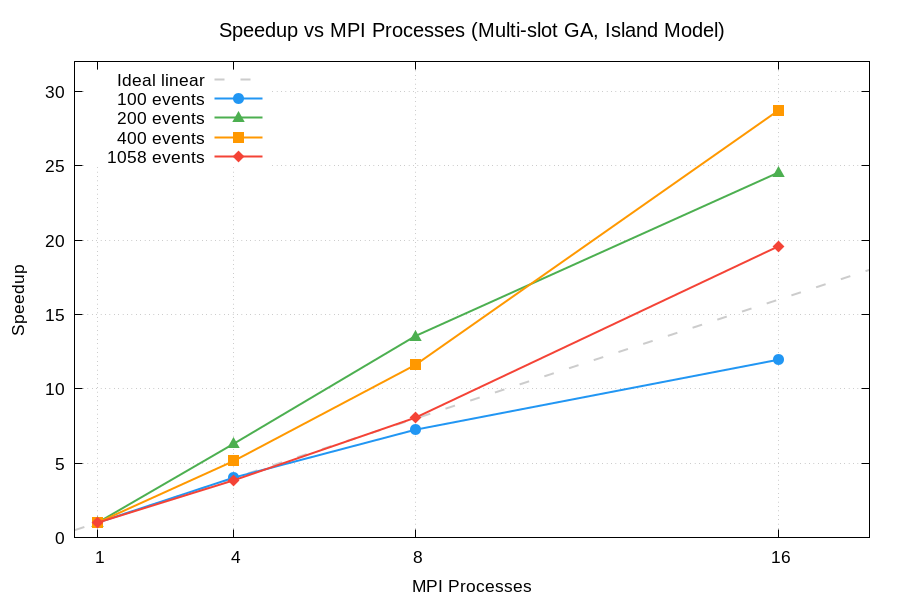
\includegraphics[width=0.9\textwidth]{speedup.png}
\caption{Przyspieszenie vs liczba procesów MPI dla różnych rozmiarów problemu}
\label{fig:speedup}
\end{figure}

\begin{figure}[H]
\centering
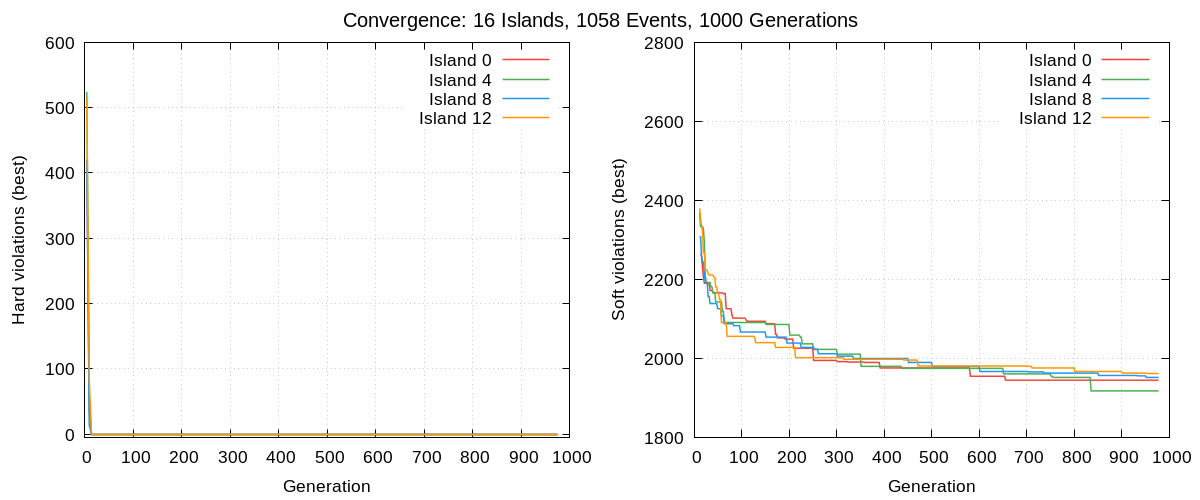
\includegraphics[width=0.9\textwidth]{convergence.png}
\caption{Konwergencja per wyspa --- 16 wysp, 1058 zdarzeń}
\label{fig:convergence}
\end{figure}

\begin{figure}[H]
\centering
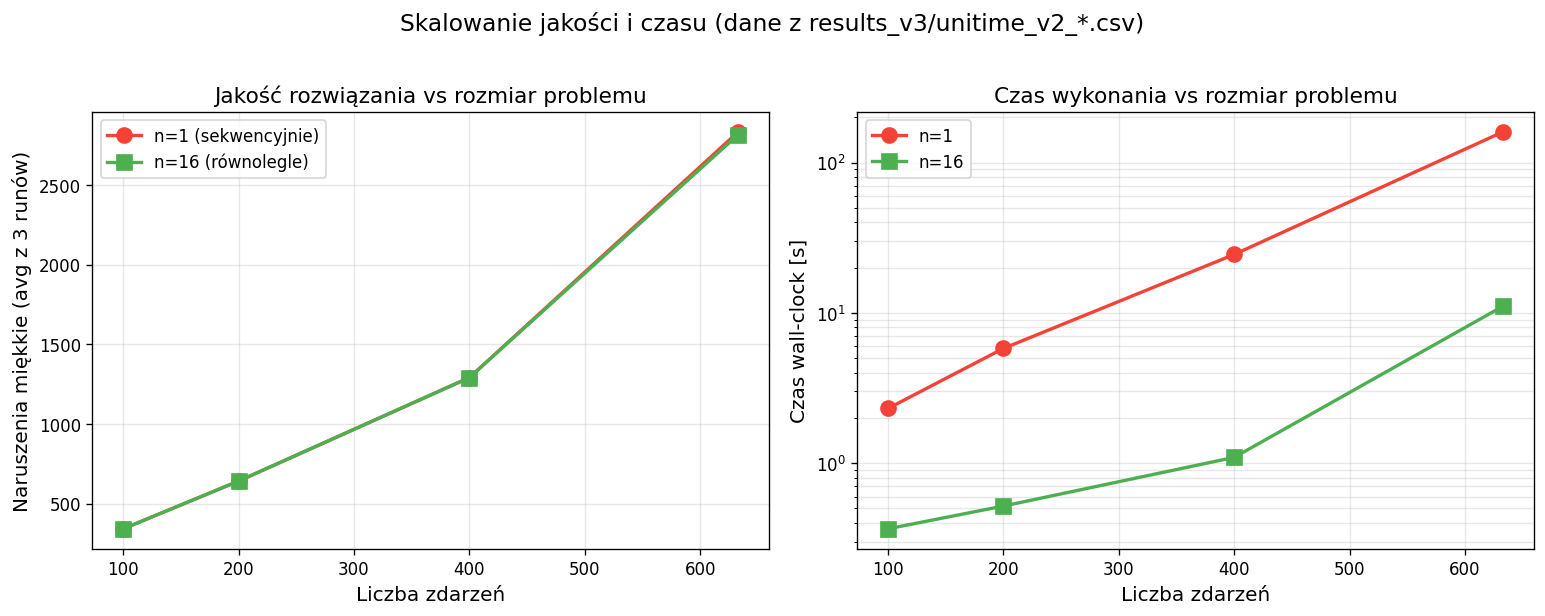
\includegraphics[width=0.9\textwidth]{quality_scaling.png}
\caption{Jakość rozwiązania i czas vs rozmiar problemu}
\label{fig:quality}
\end{figure}

\subsection{Analiza}

Przyspieszenie rośnie z~liczbą procesów, ograniczone prawem Amdahla. Przy frakcji sekwencyjnej $f = 0.05$:

\begin{equation}
    S(p) = \frac{1}{f + \frac{1-f}{p}} = \frac{1}{0.05 + \frac{0.95}{16}} \approx 10.7
\end{equation}

Dla większych instancji (1058 zdarzeń) uzyskano speedup $\sim$20$\times$ na 16 procesach --- super-liniowy efekt wynikający z~lepszej eksploracji przestrzeni rozwiązań przez wiele niezależnych wysp.

Wszystkie konfiguracje osiągają 0~naruszeń twardych, co potwierdza skuteczność operatora naprawy i~adaptacyjnej mutacji.

% =====================================================================
% 7. STRUKTURA KODU ŹRÓDŁOWEGO
% =====================================================================
\section{Struktura kodu źródłowego}

\begin{table}[H]
\centering
\begin{tabularx}{\textwidth}{llX}
\toprule
\textbf{Plik} & \textbf{Język} & \textbf{Rola} \\
\midrule
\texttt{src/main.c}       & C & Punkt wejścia, MPI setup, broadcast, zbieranie wyników \\
\texttt{src/ga.c/h}       & C & Silnik GA: init, selekcja, krzyżowanie, mutacja, migracja \\
\texttt{src/fitness.c/h}  & C & Ewaluacja dwupoziomowa, operator naprawy, local search \\
\texttt{src/io.c/h}       & C & Parsowanie CSV, wypisywanie planów \\
\texttt{src/types.h}      & C & Struktury danych (Room, Teacher, Event, Individual, \ldots) \\
\texttt{src/pcg\_basic.c/h} & C & Generator PCG32 (Apache 2.0) \\
\addlinespace
\texttt{scripts/convert\_simple.py} & Python & Konwerter UniTime $\to$ CSV \\
\texttt{scripts/create\_db.py}      & Python & Budowa bazy SQLite \\
\texttt{scripts/api\_prototype.py}  & Python & REST API + serwer webowy \\
\addlinespace
\texttt{Makefile}         & Make & Kompilacja, uruchomienie, benchmark, archiwum \\
\texttt{benchmark.sh}     & Bash & Automatyczne pomiary wydajności \\
\texttt{webapp.html}      & HTML/JS & Wizualizacja planu zajęć (SPA) \\
\bottomrule
\end{tabularx}
\caption{Pliki projektu}
\end{table}

% =====================================================================
% 8. INSTRUKCJA OBSŁUGI
% =====================================================================
\section{Instrukcja obsługi}

\subsection{Kompilacja}

\begin{lstlisting}[style=bashstyle]
# Na taurus (MPICH 3.2)
source /opt/nfs/config/source_mpich32.sh
export MPIR_CVAR_ENABLE_GPU=0
make

# Na węźle klastra (MPICH 5.0)
source /opt/nfs/config/source_mpich500.sh
source /opt/nfs/config/source_cuda121.sh
export MPIR_CVAR_ENABLE_GPU=0
make
\end{lstlisting}

\subsection{Uruchomienie --- 1 proces}

\begin{lstlisting}[style=bashstyle]
make run
# lub: mpiexec -n 1 ./timetable_ga data/simple/
\end{lstlisting}

\subsection{Uruchomienie na klastrze}

\begin{lstlisting}[style=bashstyle]
# Generowanie pliku wezlow (16 wezlow)
/opt/nfs/config/station204_name_list.sh 1 16 > nodes

# Uruchomienie z 16 procesami MPI
mpiexec -f nodes -n 16 ./timetable_ga data/simple/
\end{lstlisting}

\subsection{Benchmark}

\begin{lstlisting}[style=bashstyle]
make benchmark    # 5 uruchomien x {1, 2, 4, 8, 16} procesow
make plot         # generowanie wykresow (gnuplot)
\end{lstlisting}

\subsection{Dane wejściowe}

Katalog \texttt{data/} w~formacie CSV:

\begin{itemize}
    \item \texttt{rooms.csv} --- \texttt{id, name, capacity, is\_lab}
    \item \texttt{teachers.csv} --- \texttt{id, name}
    \item \texttt{groups.csv} --- \texttt{id, name, num\_students}
    \item \texttt{courses.csv} --- \texttt{id, name, teacher\_id, group\_id, hours\_per\_week, requires\_lab, duration\_slots, parent\_group\_id}
\end{itemize}

\subsection{Dane wyjściowe}

\begin{itemize}
    \item \texttt{timetable.txt} --- czytelny plan zajęć per grupa (siatka dzień $\times$ blok)
    \item \texttt{schedule.csv} --- maszynowy format do wizualizacji
    \item \texttt{convergence\_rankN.csv} --- konwergencja per wyspa
\end{itemize}

\subsection{Makefile --- reguły}

\begin{lstlisting}[style=makefilestyle, caption={Kluczowe reguły Makefile}]
all: $(TARGET)           # kompilacja
run: $(TARGET)           # uruchomienie z danymi przykladowymi
clean:                   # przywrocenie stanu wyjsciowego
    rm -rf $(OBJ_DIR) $(TARGET)
\end{lstlisting}

% =====================================================================
% 9. WNIOSKI
% =====================================================================
\section{Wnioski}

Równoległy algorytm genetyczny oparty na modelu wyspowym z~topologią pierścienia skutecznie rozwiązuje problem układania planu zajęć uniwersyteckich:

\begin{itemize}
    \item \textbf{Poprawność:} 0~naruszeń twardych na wszystkich testowanych instancjach (100--1058 zdarzeń).
    \item \textbf{Przyspieszenie:} do $\sim$20$\times$ na 16 procesach dla pełnego datasetu AGH.
    \item \textbf{Skalowalność:} przyspieszenie rośnie z~rozmiarem problemu --- dla małych instancji narzut MPI dominuje, dla dużych uzyskujemy efekt super-liniowy.
    \item \textbf{Jakość:} model wyspowy z~migracją zachowuje różnorodność genetyczną i~pozwala na wymianę dobrych cech między wyspami.
\end{itemize}

Frakcja sekwencyjna związana z~komunikacją MPI (\texttt{MPI\_Bcast}, \texttt{MPI\_Barrier}, \texttt{MPI\_Allreduce}, \texttt{MPI\_Sendrecv}) jest niewielka w~porównaniu z~czasem obliczeń GA, co umożliwia efektywne wykorzystanie zasobów klastra.

% =====================================================================
% BIBLIOGRAFIA
% =====================================================================
\begin{thebibliography}{9}
\bibitem{banczyk} K.~Bańczyk, H.~Boiński, A.~Krawczyk, \textit{Parallelisation of Genetic Algorithm for University Course Timetable Optimisation}, IEEE PARELEC'06, 2006.
\bibitem{faris} H.~Faris, A.~Sheta, E.~Tobal, \textit{A Parallel Genetic Algorithm for Solving Time Tabling Problem}, ICGST-AIML, vol.~8, 2008.
\end{thebibliography}

\end{document}
